\chapter{Theoretical Foundation}

If your work is based on other scientific theories and models, it is important to outline their structure and results. Use illustrations of models and theories as demonstrated below in Figure \ref{fig1}

\begin{figure}[H]
\centering
  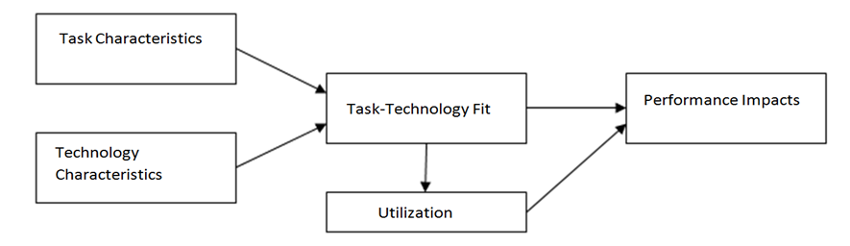
\includegraphics[width=0.5\textwidth]{grafiken/fig1}
   \caption{A picture of the universe!}
   \label{fig1}
\end{figure}


In addition to figures, one of the most powerful ways to present information in a coherent way is to create tables as shown in \ref{tab:table-name}. Make sure to include an empty line above tables and figures.
\begin{center}
\begin{table}[H]
\begin{tabularx}{\textwidth}{|X|X|X|}
\hline
Input & Output& Action return \\
\hline
DNF &  simulation & jsp\\
\hline
\end{tabularx}
\caption{\label{tab:table-name}Your caption.}
\end{table}
\end{center}


Multiple ways of presenting information can be chosen, e.g.

\begin{list}{•}{}
\item figures,
\item tables,
\item ordered lists,
\item and enumerations like this one. Here, items can be single sentences or full paragraphs. Appropriate end punctuation should be included.

\end{list}

